%\usepackage[spanish]{babel}
\chapter{Introducción}

En esta etapa de la validación se presentan los resultados correspondientes a la ejecución de pruebas en los sistemas computarizados Agilent OpenLAB CDS (EZChrom Edition), Perkin Elmer TotalChrom navigator y Bettersize laser size particle analyzer. El proposito del test es organizar los \textit{casos de prueba} en procedimientos y realizar las pruebas físicas de cada \textit{escenario de uso} en el ambiente correcto. Este nivel es ejecutado por el equipo de pruebas en conjunto con los expertos de dominio en conformidad con las politicas de acceso, protocolos de persistencia e integridad de datos.

\chapter{Ejecución de las pruebas}

\subsubsection{Métrica de resultado}

\begin{table}[H]
	\begin{center}
		\begin{tabular}{| p{3cm} | p{7cm} | p{1cm} |}
			\hline
			Resultado & Definición & Sigla \\
			\hline \hline
			Error Humano & Acción Humana que produce un resultado incorrecto & M \\ \hline
			Defecto & Paso, proceso o definición de datos incorrecto & D \\ \hline
			Falla &la incapacidad de un componente para realizar la función requerida
			dentro de los requisitos de funcionamiento especificados.  & F \\ \hline
			Error & Diferencia entre el valor medido y el teorico & E \\ \hline
			No aplica & Sin hallazgos & n/a \\ \hline
		\end{tabular}
		\caption{Métricas de evaluación}
		\label{tabla:sencilla}
	\end{center}
\end{table}

\section{Pruebas funcionales - Agilent Openlab EZChrom }

\subsection{CRUD método}

\begin{figure}[H]
	\centering
	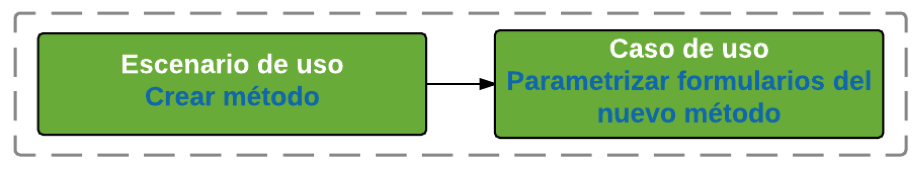
\includegraphics[width=0.7\linewidth]{img/crearmetodo.png}
	\caption{Prueba funcional Agilent - Crear método}
	\label{fig:MarcoTeorico}
\end{figure}

\begin{table}[H]
	\begin{center}
		\begin{tabular}{|l|l|}
			\hline
			Procedimiento de prueba & 1.1\\
			\hline \hline
			Sistema & Agilent OpenLAB EZChrom Edition V: A.04.07 \\ \hline
			Escenario de uso & Crear método\\ \hline
			Caso de uso & Parametrizar formulario \\ \hline
			Duración esperada & 5 min\\ \hline
			Muestra & Test\\ \hline
			Datos de entrada & Column Oven, Grad. Pump, DAD, Sampler\\ \hline
			Salida esperada  & Método creado\\ \hline	
			Salida actual & Método creado\\ \hline	
			Resultado & n/a\\ \hline
			\end{tabular}
		\caption{Registro de prueba Agilent - Crear método}
		\label{tabla:sencilla}
	\end{center}
\end{table}

\begin{figure}[H]
	\centering
	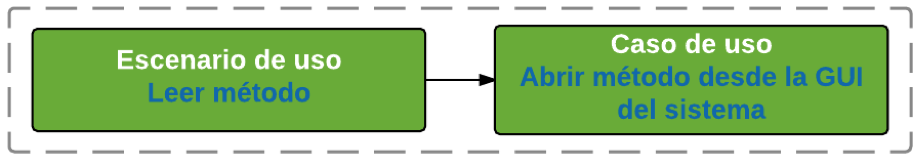
\includegraphics[width=0.7\linewidth]{img/leermetodo.png}
	\caption{Prueba funcional Agilent - Leer método}
	\label{fig:MarcoTeorico}
\end{figure}

\begin{table}[H]
	\begin{center}
		\begin{tabular}{|l|l|}
			\hline
			Procedimiento de prueba & 1.2\\
			\hline \hline
			Sistema & Agilent OpenLAB EZChrom Edition V: A.04.07 \\ \hline
			Escenario de uso & Leer método\\ \hline
			Caso de uso & Parametrizar formulario \\ \hline
			Duración esperada & 1 min\\ \hline
			Muestra & Test\\ \hline
			Datos de entrada & test.met\\ \hline
			Salida esperada  & Lectura del método\\ \hline	
			Salida actual & Método en lectura\\ \hline	
			Resultado & n/a\\ \hline
		\end{tabular}
		\caption{Registro de prueba Agilent - Leer método}
	\label{tabla:sencilla}
\end{center}
\end{table}
\newpage
\begin{figure}[H]
	\centering
	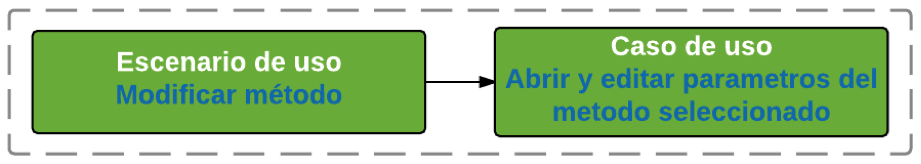
\includegraphics[width=0.7\linewidth]{img/modificarmetodo.png}
	\caption{Prueba funcional Agilent - Editar método}
	\label{fig:MarcoTeorico}
\end{figure}

\begin{table}[H]
	\begin{center}
	\begin{tabular}{|l|l|}
	\hline
	Procedimiento de prueba & 1.3\\
	\hline \hline
	Sistema & Agilent OpenLAB EZChrom Edition V: A.04.07 \\ \hline
	Escenario de uso & Editar método\\ \hline
	Caso de uso & Parametrizar formulario \\ \hline
	Duración esperada & 5 min\\ \hline
	Muestra & Test\\ \hline
	Datos de entrada & test.met, Column Oven, Grad. Pump, DAD, Sampler\\ \hline
	Salida esperada  & Método editado\\ \hline	
	Salida actual & Método editado\\ \hline	
	Resultado & n/a\\ \hline
\end{tabular}
		\caption{Registro de prueba Agilent - Modificar método}
		\label{tabla:sencilla}
	\end{center}
\end{table}
\newpage
\begin{figure}[H]
	\centering
	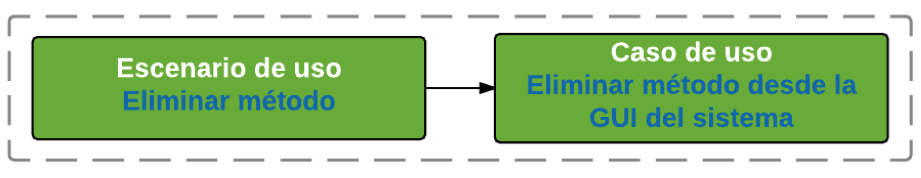
\includegraphics[width=0.7\linewidth]{img/eliminarmetodo.png}
	\caption{Prueba funcional Agilent - Eliminar método}
	\label{fig:MarcoTeorico}
\end{figure}

\begin{table}[H]
	\begin{center}
		\begin{tabular}{|l|l|}
		\hline
		Procedimiento de prueba & 1.4\\
		\hline \hline
		Sistema & Agilent OpenLAB EZChrom Edition V: A.04.07 \\ \hline
		Escenario de uso & Crear método\\ \hline
		Caso de uso & Parametrizar formulario \\ \hline
		Duración esperada & 5 min\\ \hline
		Muestra & Test\\ \hline
		Datos de entrada & test.met\\ \hline
		Salida esperada  & Método eliminado\\ \hline	
		Salida actual & Método eliminado\\ \hline	
		Resultado & n/a\\ \hline
	\end{tabular}
		\caption{Registro de prueba Agilent - Eliminar método}
		\label{tabla:sencilla}
	\end{center}
\end{table}

\subsection{CRUD secuencia}

\begin{figure}[H]
	\centering
	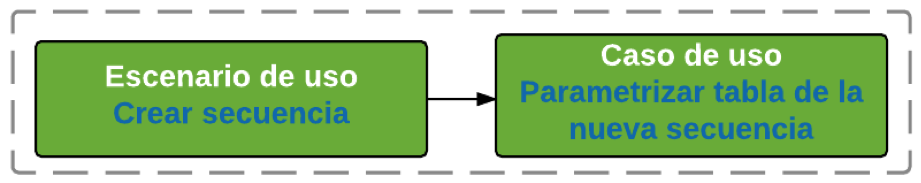
\includegraphics[width=0.7\linewidth]{img/crearsecuencia.png}
	\caption{Prueba funcional Agilent - Crear secuencia}
	\label{fig:MarcoTeorico}
\end{figure}

\begin{table}[H]
	\begin{center}
		\begin{tabular}{|l|l|}
			\hline
			Procedimiento de prueba & 1.5\\
			\hline \hline
			Sistema & Agilent OpenLAB EZChrom Edition V: A.04.07 \\ \hline
			Escenario de uso & Crear secuencia \\ \hline
			Caso de uso & Parametrizar tabla \\ \hline
			Duración esperada & 5 min \\ \hline
			Muestra & Test \\ \hline
			Datos de entrada & Run type, Level, Reps, test.met \\ \hline
			Salida esperada  & Secuencia creada\\ \hline	
			Salida actual & Secuencia creada\\ \hline	
			Resultado & n/a\\ \hline
		\end{tabular}
		\caption{Registro de prueba Agilent - Crear Secuencia}
		\label{tabla:sencilla}
	\end{center}
\end{table}

\begin{figure}[H]
	\centering
	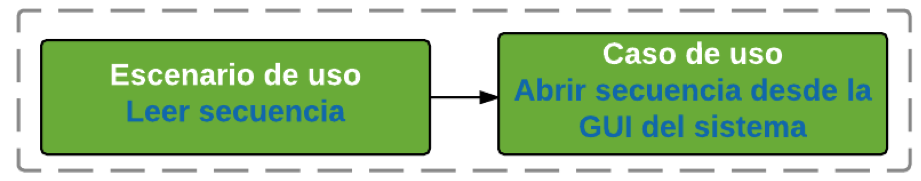
\includegraphics[width=0.7\linewidth]{img/leersecuencia.png}
	\caption{Prueba funcional Agilent - Leer secuencia}
	\label{fig:MarcoTeorico}
\end{figure}

\begin{table}[H]
	\begin{center}
		\begin{tabular}{|l|l|}
			\hline
			Procedimiento de prueba & 1.6\\
			\hline \hline
			Sistema & Agilent OpenLAB EZChrom Edition V: A.04.07\\ \hline
			Escenario de uso & Leer secuencia \\ \hline
			Caso de uso & Abrir secuencia desde la GUI\\ \hline
			Duración esperada & 1 min\\ \hline
			Muestra & Test\\ \hline
			Datos de entrada & test.sec\\ \hline
			Salida esperada  & Lectura de una secuencia\\ \hline	
			Salida actual & Secuencia en lectura\\ \hline	
			Resultado & n/a \\ \hline
		\end{tabular}
		\caption{Registro de prueba Agilent - Leer secuencia}
		\label{tabla:sencilla}
	\end{center}
\end{table}
\newpage
\begin{figure}[H]
	\centering
	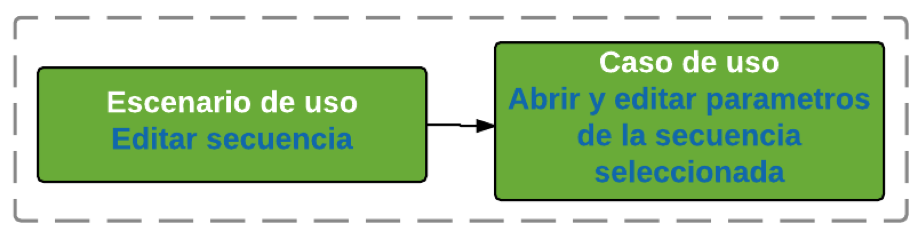
\includegraphics[width=0.7\linewidth]{img/editarsecuencia.png}
	\caption{Prueba funcional Agilent - Editar secuencia}
	\label{fig:MarcoTeorico}
\end{figure}

\begin{table}[H]
	\begin{center}
		\begin{tabular}{|l|l|}
			\hline
			Procedimiento de prueba & 1.7\\
			\hline \hline
			Sistema & Agilent OpenLAB EZChrom Edition V: A.04.07\\ \hline
			Escenario de uso &Editar secuencia \\ \hline
			Caso de uso & editar parametros de la secuencia \\ \hline
			Duración esperada & 5 min \\ \hline
			Muestra & Test \\ \hline
			Datos de entrada & test.sec\\ \hline
			Salida esperada  & Secuencia editada\\ \hline	
			Salida actual & Secuencia editada\\ \hline	
			Resultado & n/a\\ \hline
		\end{tabular}
		\caption{Registro de prueba Agilent - Editar secuencia}
		\label{tabla:sencilla}
	\end{center}
\end{table}
\newpage
\begin{figure}[H]
	\centering
	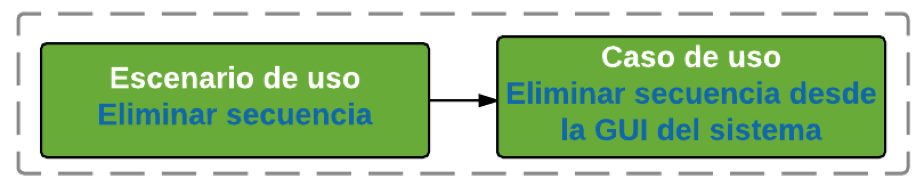
\includegraphics[width=0.7\linewidth]{img/eliminarsecuencia.png}
	\caption{Prueba funcional Agilent - Eliminar secuencia}
	\label{fig:MarcoTeorico}
\end{figure}

\begin{table}[H]
	\begin{center}
		\begin{tabular}{|l|l|}
			\hline
			Procedimiento de prueba & 1.8\\
			\hline \hline
			Sistema & Agilent OpenLAB EZChrom Edition V: A.04.07\\ \hline
			Escenario de uso & Eliminar secuencia\\ \hline
			Caso de uso & Eliminar secuencia desde la GUI \\ \hline
			Duración esperada & 1 min\\ \hline
			Muestra & Test\\ \hline
			Datos de entrada & test.sec\\ \hline
			Salida esperada  & Secuencia eliminada\\ \hline	
			Salida actual & Secuencia eliminada\\ \hline	
			Resultado & n/a \\ \hline
		\end{tabular}
		\caption{Registro de prueba Agilent - Eliminar secuencia}
		\label{tabla:sencilla}
	\end{center}
\end{table}
\newpage
\subsection{Prueba de aceptación - Agilent OpenLAB EZChrom}

El objetivo de este nivel es verificar el cumplimiento de los requerimientos de usuario mediante una prueba que integre la aplicación de los \textit{escenarios de uso}, en un procedimiento de rutina, bajo condiciones normales de operación.

\begin{itemize}
\item \textbf{Requerimiento}: Comparar las muestras de planta (Desarrollo y producción) con muestras estándar, con el fin asegurar las concentraciones de ingredientes activos.
\item \textbf{Muestras}: Flutriafol/Flutriafol STD.
\end{itemize}

\subsubsection{Parametrizar método}

\begin{itemize}
	\item El experto de dominio crea un método y de define sus parametros [Figura 2.9] que correspondan a la muestra \textbf{(lutriafol/Flutriafol STD)}.
	
\end{itemize}

\begin{figure}[H]
	\centering
	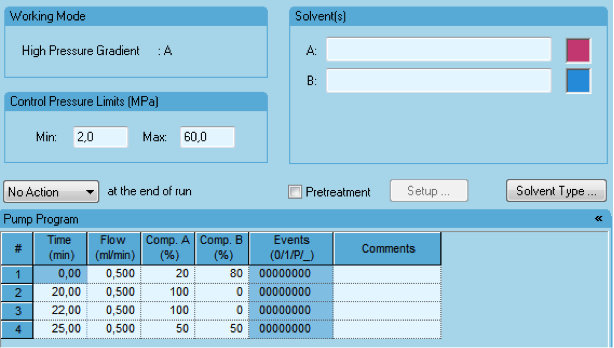
\includegraphics[width=0.45\linewidth]{img/aceptacion1.png}
	\caption{Configuración del método}
	\label{fig:MarcoTeorico}
\end{figure}

\subsubsection{Ejecutar secuencia}

\begin{itemize}
	\item El experto de domonio ejecuta la secuencia haciendo uso del método definido anteriormente [Figura 2.10].
\end{itemize}

\begin{figure}[H]
	\centering
	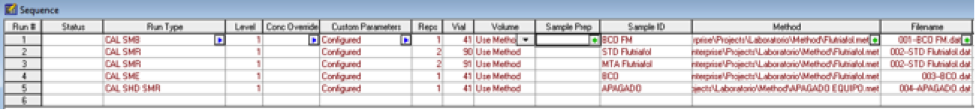
\includegraphics[width=0.9\linewidth]{img/aceptacion2.png}
	\caption{Configuración y ejecución de la secuencia}
	\label{fig:MarcoTeorico}
\end{figure}

\subsubsection{Reprocesar datos}



\begin{figure}[H]
	\centering
	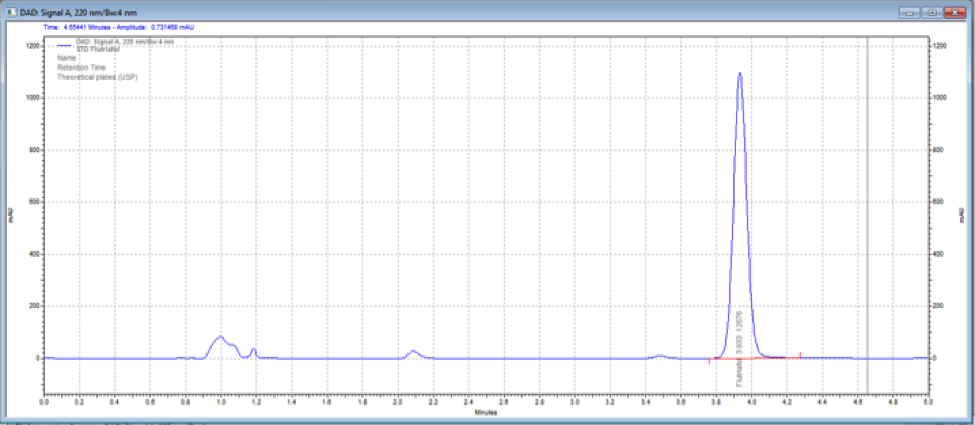
\includegraphics[width=0.5\linewidth]{img/aceptacion3.png}
	\caption{Obtención del cromatograma}
	\label{fig:MarcoTeorico}
\end{figure}
\subsubsection{Reporte}

\begin{itemize}
	\item Se configuran los parametros de integración [Figura 2.23] y se reprocesan los datos, finalmente se muestra información pertinente al análisis en un formato estándar [Figura 2.24] .
\end{itemize}

\begin{figure}[H]
	\centering
	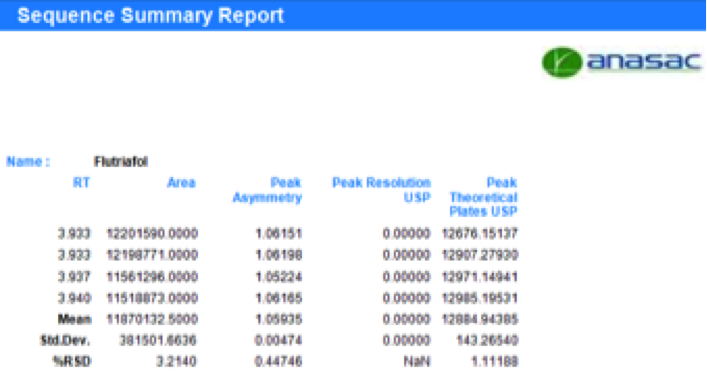
\includegraphics[width=0.4\linewidth]{img/aceptacion4.png}
	\caption{Visa de los resultados}
	\label{fig:MarcoTeorico}
\end{figure}

\subsubsection{Estado de la validación: El sistema satisface el requerimiento}
\newpage
\section{Pruebas funcionales - GC TotalChrom navigator}

\subsubsection{Nota}

Se requiere la reinstalación del sistema operativo (Windows 7 sp1 x64) ya que se encuentra en mal estado, debido al funcionamiento, por uso incorrecto (Malas prácticas).
La interacción con los equipos debe ser de uso exclusivo, acorde a politicas de acceso y operaciones previstas, con el fin de no acortar la vida útil del sistema en anfitrión (Microsoft Windows).

\subsection{CRUD método}

\begin{figure}[H]
	\centering
	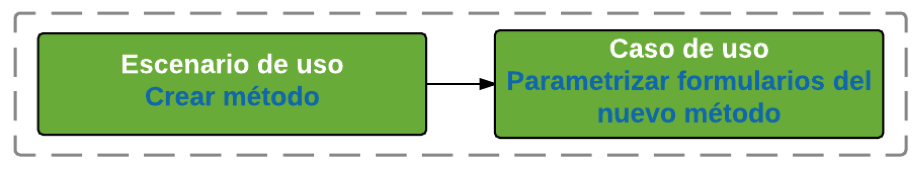
\includegraphics[width=0.7\linewidth]{img/crearmetodo.png}
	\caption{Prueba funcional GC - Crear método}
	\label{fig:MarcoTeorico}
\end{figure}

\begin{table}[H]
	\begin{center}
		\begin{tabular}{|l|l|}
			\hline
			Procedimiento de prueba & 2.1\\
			\hline \hline
			Sistema & GC TotalChrom navigator\\ \hline
			Escenario de uso & Crear método \\ \hline
			Caso de uso & Parametrizar formulario \\ \hline
			Duración esperada & 1 min\\ \hline
			Muestra & Test \\ \hline
			Datos de entrada &  \\ \hline
			Salida esperada  & Método creado\\ \hline	
			Salida actual & Método creado\\ \hline	
			Resultado & n/a \\ \hline
		\end{tabular}
		\caption{Registro de prueba GC - Crear método}
		\label{tabla:sencilla}
	\end{center}
\end{table}

\begin{figure}[H]
	\centering
	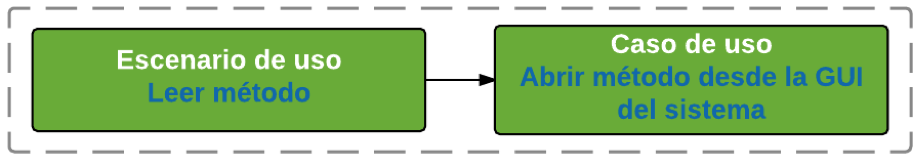
\includegraphics[width=0.7\linewidth]{img/leermetodo.png}
	\caption{Prueba funcional GC - Leer método}
	\label{fig:MarcoTeorico}
\end{figure}

\begin{table}[H]
	\begin{center}
		\begin{tabular}{|l|l|}
			\hline
			Procedimiento de prueba & 2.2\\
			\hline \hline
			Sistema & GC TotalChrom navigator \\ \hline
			Escenario de uso & Leer métodod\\ \hline
			Caso de uso & Abrir método \\ \hline
			Duración esperada & 1 min \\ \hline
			Muestra & Test \\  \hline
			Datos de entrada & test.met\\ \hline
			Salida esperada  &Vista del método\\ \hline	
			Salida actual &Vista del método\\  \hline	
			Resultado & n/a \\ \hline
		\end{tabular}
		\caption{Registro de prueba GC - Leer método}
		\label{tabla:sencilla}
	\end{center}
\end{table}
\newpage
\begin{figure}[H]
	\centering
	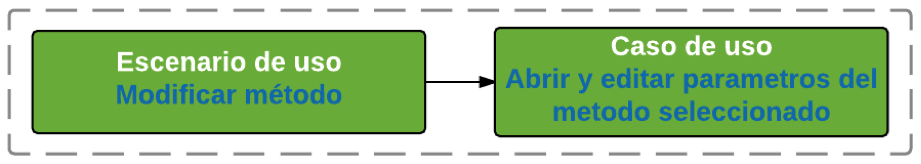
\includegraphics[width=0.7\linewidth]{img/modificarmetodo.png}
	\caption{Prueba funcional GC - Editar método}
	\label{fig:MarcoTeorico}
\end{figure}

\begin{table}[H]
	\begin{center}
		\begin{tabular}{|l|l|}
			\hline
			Procedimiento de prueba & 2.3\\
			\hline \hline
			Sistema & GC TotalChrom navigator \\ \hline
			Escenario de uso & Modificar método\\  \hline
			Caso de uso & Abrir y editar parametros \\ \hline
			Duración esperada & 1 min\\  \hline
			Muestra & Test\\\hline
			Datos de entrada & test.met\\  \hline
			Salida esperada  &Método editado\\  \hline	
			Salida actual &Método editado\\ \hline	
			Resultado & n/a \\\hline
		\end{tabular}
		\caption{Registro de prueba GC - Editar método}
		\label{tabla:sencilla}
	\end{center}
\end{table}
\newpage
\begin{figure}[H]
	\centering
	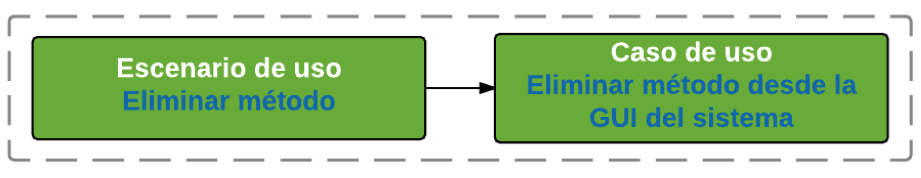
\includegraphics[width=0.7\linewidth]{img/eliminarmetodo.png}
	\caption{Prueba funcional GC - Eliminar método}
	\label{fig:MarcoTeorico}
\end{figure}

\begin{table}[H]
	\begin{center}
		\begin{tabular}{|l|l|}
			\hline
			Procedimiento de prueba & 2.4\\
			\hline \hline
			Sistema & GC TotalChrom navigator\\ \hline
			Escenario de uso &  Eliminar método \\ \hline
			Caso de uso &  Eliminar método\\  \hline
			Duración esperada & 1 min \\  \hline
			Muestra & Test  \\  \hline
			Datos de entrada & test.met\\  \hline
			Salida esperada  & Método eliminado \\  \hline	
			Salida actual & Método eliminado \\  \hline	
			Resultado & n/a \\  \hline
		\end{tabular}
		\caption{Registro de prueba GC - Eliminar método}
		\label{tabla:sencilla}
	\end{center}
\end{table}

\subsection{CRUD secuencia}

\begin{figure}[H]
	\centering
	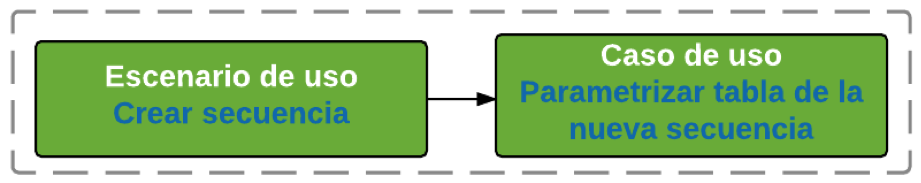
\includegraphics[width=0.7\linewidth]{img/crearsecuencia.png}
	\caption{Prueba funcional GC - Crear secuencia}
	\label{fig:MarcoTeorico}
\end{figure}

\begin{table}[H]
	\begin{center}
		\begin{tabular}{|l|l|}
			\hline
			Procedimiento de prueba & 2.5\\
			\hline \hline
			Sistema & GC TotalChrom navigator \\ \hline
			Escenario de uso & Crear secuencia \\  \hline
			Caso de uso & Parametrizar tabla \\  \hline
			Duración esperada & 1 min\\ \hline
			Muestra & Test \\ \hline
			Datos de entrada & test.met\\ \hline
			Salida esperada  & Nueva secuencia\\  \hline	
			Salida actual & Nueva secuencia \\ \hline	
			Resultado & n/a \\ \hline
		\end{tabular}
		\caption{Registro de prueba GC - Crear secuencia}
		\label{tabla:sencilla}
	\end{center}
\end{table}

\begin{figure}[H]
	\centering
	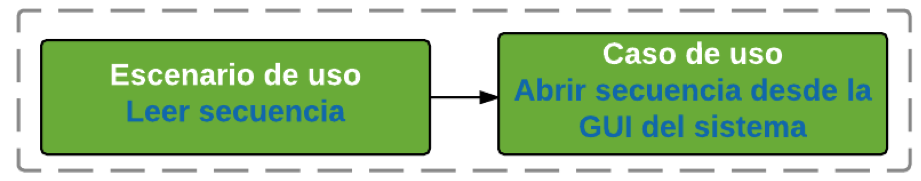
\includegraphics[width=0.7\linewidth]{img/leersecuencia.png}
	\caption{Prueba funcional GC - Leer secuencia}
	\label{fig:MarcoTeorico}
\end{figure}

\begin{table}[H]
	\begin{center}
		\begin{tabular}{|l|l|}
			\hline
			Procedimiento de prueba & 2.6\\
			\hline \hline
			Sistema & GC TotalChrom navigator \\ \hline
			Escenario de uso & Leer secuencia\\ \hline
			Caso de uso & Abrir secuencia desde la GUI \\ \hline
			Duración esperada & 1 min \\ \hline
			Muestra & Test\\ \hline
			Datos de entrada & Test.sec \\ \hline
			Salida esperada  & Vista de la secuencia\\ \hline	
			Salida actual & GC TotalChrom navigator\\ \hline	
			Resultado & n/a \\ \hline
		\end{tabular}
		\caption{Registro de prueba GC - Leer secuencia}
		\label{tabla:sencilla}
	\end{center}
\end{table}
\newpage
\begin{figure}[H]
	\centering
	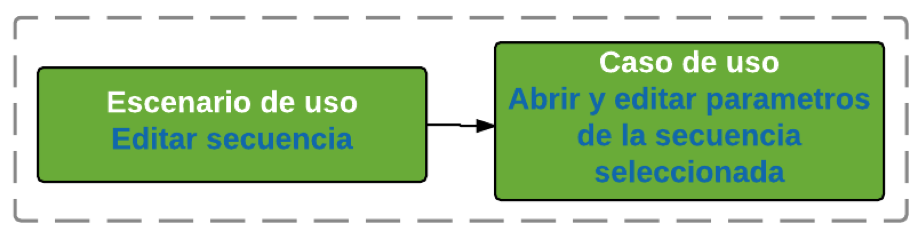
\includegraphics[width=0.7\linewidth]{img/editarsecuencia.png}
	\caption{Prueba funcional GC - Editar secuencia}
	\label{fig:MarcoTeorico}
\end{figure}

\begin{table}[H]
	\begin{center}
		\begin{tabular}{|l|l|}
			\hline
			Procedimiento de prueba & 2.7\\
			\hline \hline
			Sistema & GC TotalChrom navigator\\ \hline
			Escenario de uso & Editar secuencia \\ \hline
			Caso de uso & Abir y editar parametros  \\ \hline
			Duración esperada & 2 min\\ \hline
			Muestra & Test\\ \hline
			Datos de entrada & test.sec \\ \hline
			Salida esperada  & Secuencia editada \\ \hline	
			Salida actual & Secuencia editada\\ \hline	
			Resultado & n/a\\ \hline
		\end{tabular}
		\caption{Registro de prueba GC - Editar secuencia}
		\label{tabla:sencilla}
	\end{center}
\end{table}
\newpage
\begin{figure}[H]
	\centering
	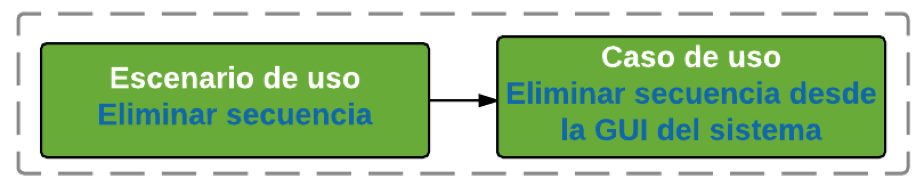
\includegraphics[width=0.7\linewidth]{img/eliminarsecuencia.png}
	\caption{Prueba funcional GC - Eliminar secuencia}
	\label{fig:MarcoTeorico}
\end{figure}

\begin{table}[H]
	\begin{center}
		\begin{tabular}{|l|l|}
			\hline
			Procedimiento de prueba & 2.8\\
			\hline \hline
			Sistema & GC TotalChrom navigator\\ \hline
			Escenario de uso & Eliminar secuencia \\ \hline
			Caso de uso & Eliminar secuencia desde la GUI \\ \hline
			Duración esperada & 1 min \\ \hline
			Muestra & Test \\ \hline
			Datos de entrada & test.met \\ \hline
			Salida esperada  & Secuencia eliminado \\ \hline	
			Salida actual & Secuencia eliminado \\ \hline	
			Resultado & n/a \\ \hline
		\end{tabular}
		\caption{Registro de prueba GC - Eliminar secuencia}
		\label{tabla:sencilla}
	\end{center}
\end{table}

\subsection{Prueba de aceptación - GC TotalChrom navigator}

El objetivo de este nivel es verificar el cumplimiento de los requerimientos de usuario mediante una prueba que integre la aplicación de los \textit{escenarios de uso}, en un procedimiento de rutina, bajo condiciones normales de operación.

\begin{itemize}
	\item \textbf{Requerimiento}: Comparar las muestras de planta (Desarrollo y producción) con muestras estándar, con el fin asegurar las concentraciones de ingredientes activos.
	\item \textbf{Muestras}: Azoxistrobin 120 + tebuconazole 200 sc.
\end{itemize}

\subsubsection{Parametrizar método}

\begin{itemize}
	\item El experto de dominio crea un método y de define sus parametros [Figura 2.21] que correspondan a la muestra \textbf{(Azoxistrobin + tebuconazole)}.
	 
\end{itemize}

\begin{figure}[H]
	\centering
	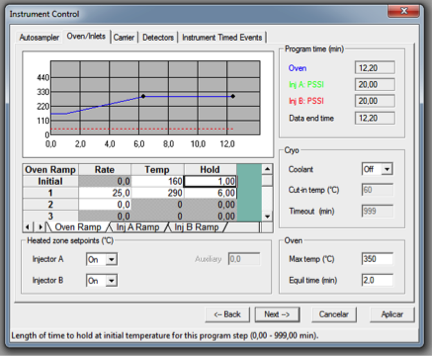
\includegraphics[width=0.5\linewidth]{img/aceptacion1_gc.png}
	\caption{Configuración del método}
	\label{fig:MarcoTeorico}
\end{figure}

\subsubsection{Ejecutar secuencia}

\begin{itemize}
	\item El experto de domonio ejecuta la secuencia haciendo uso del método definido anteriormente [Figura 2.22].
\end{itemize}

\begin{figure}[H]
	\centering
	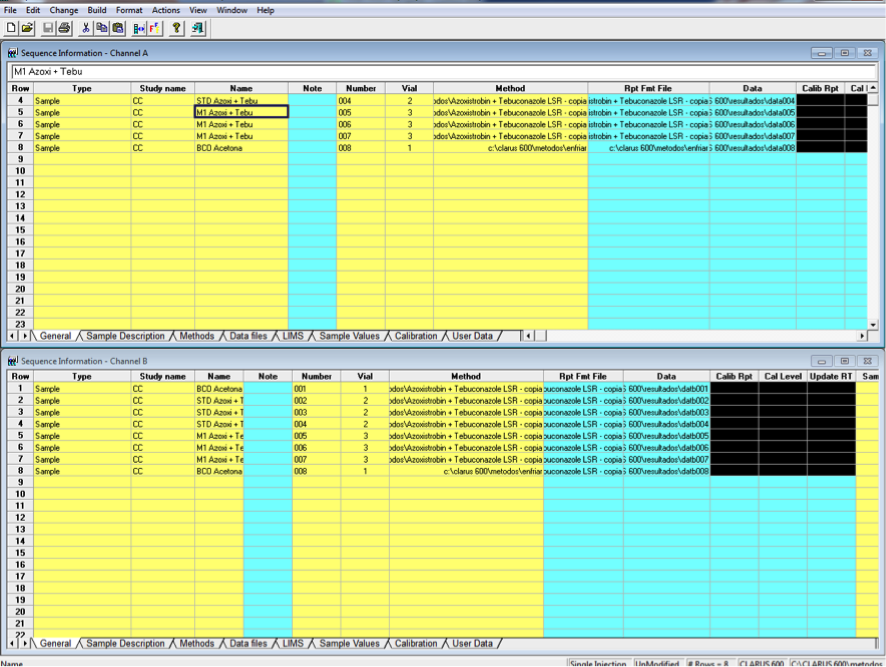
\includegraphics[width=0.7\linewidth]{img/aceptacion2_gc.png}
	\caption{Configuración y ejecución de la secuencia}
	\label{fig:MarcoTeorico}
\end{figure}

\subsubsection{Reprocesar datos}

\begin{itemize}
	\item Se configuran los parametros de integración [Figura 2.23] y se reprocesan los datos, finalmente se muestra información pertinente al análisis en un formato estándar [Figura 2.24] .
\end{itemize}

\begin{figure}[H]
	\centering
	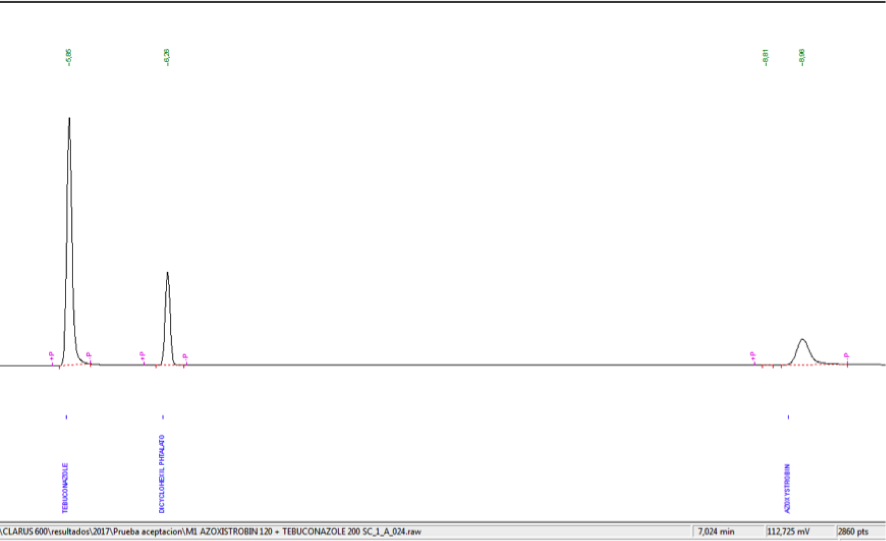
\includegraphics[width=0.7\linewidth]{img/aceptacion3_gc.png}
	\caption{Obtención del cromatograma}
	\label{fig:MarcoTeorico}
\end{figure}
\subsubsection{Reporte}

\begin{figure}[H]
	\centering
	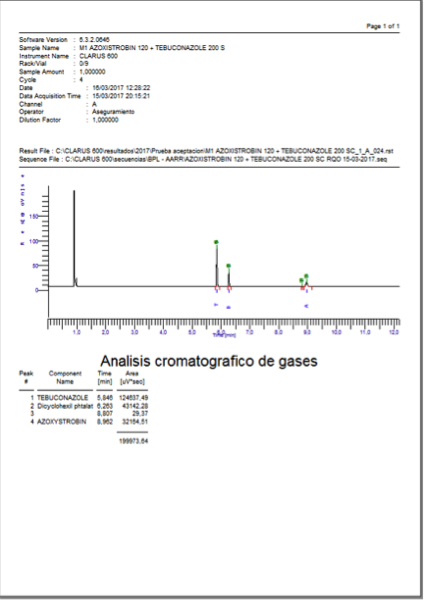
\includegraphics[width=0.6\linewidth]{img/aceptacion4_gc.png}
	\caption{Visa de los resultados}
	\label{fig:MarcoTeorico}
\end{figure}

\subsubsection{Estado de la validación: El sistema satisface el requerimiento}
\newpage

\section{Pruebas funcionales - Bettersize BT - 9300H}

\subsubsection{Nota}

Se registra una falla en el sistema durante la ejecución del \textbf{caso de uso - vista de resultados}, para las muestras [\textbf{Dixiodo de titanio STD y Diazinon 40}]. Se requiere reinstalación del software (Bettersize BT- 9300) en un ambiente limpio (Windows 7 sp1 x64) antes de la siguiente iteración.

\subsubsection{Test 1: Dioxido de titanio STD}

\begin{figure}[H]
	\centering
	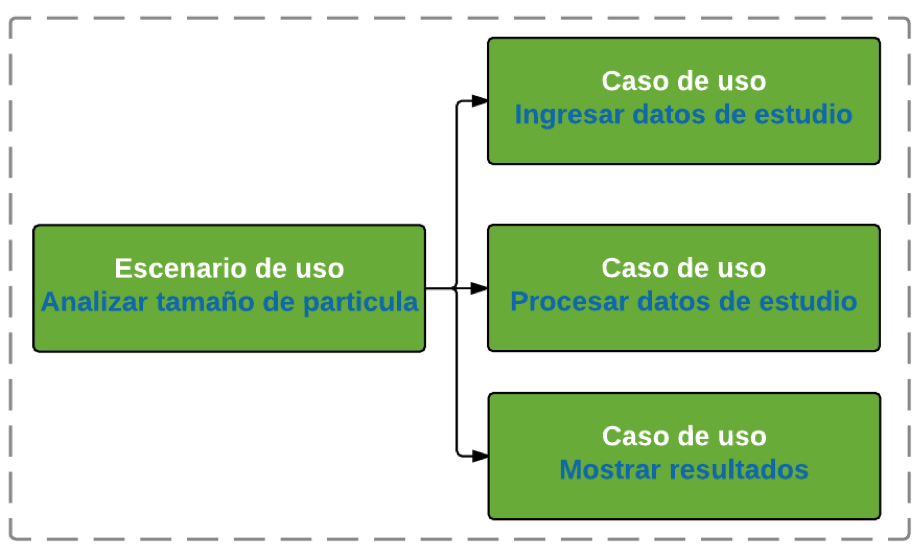
\includegraphics[width=0.6\linewidth]{img/bettersize.png}
	\caption{Analizar tamaño de partícula}
	\label{fig:MarcoTeorico}
\end{figure}

\begin{table}[H]
	\begin{center}
		\begin{tabular}{|l|l|}
			\hline
			Procedimiento de prueba & 3.1\\
			\hline \hline
			Sistema & Bettersize Laser Particle size analyzer V: 5.0 \\ \hline
			Escenario de uso & Analizar tamaño de partícula\\ \hline
			Caso de uso &  Ingresar datos de estudio \\ \hline
			Duración esperada & 5 min\\ \hline
			Muestra & Dioxido de titanio STD\\ \hline
			Datos de entrada & Sample name, Operator, Remark \\ \hline
			Salida esperada  & Datos ingresados  \\ \hline	
			Salida actual & Datos ingresados \\ \hline	
			Resultado & n/a \\ \hline
			
		\end{tabular}
		\caption{Registro de prueba Bettersize - Ingresar datos}
		\label{tabla:sencilla}
	\end{center}
\end{table}

\begin{table}[H]
	\begin{center}
		\begin{tabular}{|l|l|}
			\hline
			Procedimiento de prueba & 3.2\\
			\hline \hline
			Sistema & Bettersize Laser Particle size analyzer V: 5.0 \\ \hline
			Escenario de uso & Analizar tamaño de partícula\\ \hline
			Caso de uso & Procesar datos de estudio \\ \hline
			Duración esperada & 5 min\\ \hline
			Muestra & Dioxido de titanio STD\\ \hline
			Datos de entrada & sample.dat \\ \hline
			Salida esperada  & Datos procesados \\ \hline	
			Salida actual & Datos procesados \\ \hline	
			Resultado & n/a \\ \hline
			
		\end{tabular}
		\caption{Registro de prueba Bettersize - Procesar datos}
		\label{tabla:sencilla}
	\end{center}
\end{table}

\begin{table}[H]
	\begin{center}
		\begin{tabular}{|l|l|}
			\hline
			Procedimiento de prueba & 3.3\\
			\hline \hline
			Sistema & Bettersize Laser Particle size analyzer V: 5.0 \\ \hline
			Escenario de uso & Analizar tamaño de partícula\\ \hline
			Caso de uso & Mostrar resultados \\ \hline
			Duración esperada & 1 min\\ \hline
			Muestra & Dioxido de titanio STD\\ \hline
			Datos de entrada & sample.dat \\ \hline
			Salida esperada (size) & [0,82 - 1,22] unidades \\ \hline	
			Salida actual & [0] unidades\\ \hline	
			Resultado & F \\ \hline
		\end{tabular}
		\caption{Registro de prueba Bettersize - Vista resultados}
		\label{tabla:sencilla}
	\end{center}
\end{table}

\subsubsection{Test 2: Diozinon 40WP}

\begin{table}[H]
	\begin{center}
		\begin{tabular}{|l|l|}
			\hline
			Procedimiento de prueba & 3.1\\
			\hline \hline
			Sistema & Bettersize Laser Particle size analyzer V: 5.0 \\ \hline
			Escenario de uso & Analizar tamaño de partícula\\ \hline
			Caso de uso &  Ingresar datos de estudio \\ \hline
			Duración esperada & 5 min\\ \hline
			Muestra & Diazinon 40 WP\\ \hline
			Datos de entrada & Sample name, Operator, Remark \\ \hline
			Salida esperada  & Datos ingresados  \\ \hline	
			Salida actual & Datos ingresados \\ \hline	
			Resultado & n/a \\ \hline
			
		\end{tabular}
		\caption{Registro de prueba Bettersize - Ingresar datos}
		\label{tabla:sencilla}
	\end{center}
\end{table}

\begin{table}[H]
	\begin{center}
		\begin{tabular}{|l|l|}
			\hline
			Procedimiento de prueba & 3.2\\
			\hline \hline
			Sistema & Bettersize Laser Particle size analyzer V: 5.0 \\ \hline
			Escenario de uso & Analizar tamaño de partícula\\ \hline
			Caso de uso & Procesar datos de estudio \\ \hline
			Duración esperada & 5 min\\ \hline
			Muestra & Diazinon 40 WP\\ \hline
			Datos de entrada & sample.dat \\ \hline
			Salida esperada  & Datos procesados \\ \hline	
			Salida actual & Datos procesados \\ \hline	
			Resultado & n/a \\ \hline
			
		\end{tabular}
		\caption{Registro de prueba Bettersize - Procesar datos}
		\label{tabla:sencilla}
	\end{center}
\end{table}

\begin{table}[H]
	\begin{center}
		\begin{tabular}{|l|l|}
			\hline
			Procedimiento de prueba & 3.3\\
			\hline \hline
			Sistema & Bettersize Laser Particle size analyzer V: 5.0 \\ \hline
			Escenario de uso & Analizar tamaño de partícula\\ \hline
			Caso de uso & Mostrar resultados \\ \hline
			Duración esperada & 1 min\\ \hline
			Muestra & Dioxido de titanio STD\\ \hline
			Datos de entrada & sample.dat \\ \hline
			Salida esperada (size) & [0,1 - 40] unidades \\ \hline	
			Salida actual & [0] unidades\\ \hline	
			Resultado & F \\ \hline
		\end{tabular}
		\caption{Registro de prueba Bettersize - Vista resultados}
		\label{tabla:sencilla}
	\end{center}
\end{table}

\subsection{Prueba de aceptación - Bettersize BT - 9300H}

El objetivo de este nivel es verificar el cumplimiento de los requerimientos de usuario mediante una prueba que integre la aplicación de los \textit{escenarios de uso}, en un procedimiento de rutina, bajo condiciones normales de operación.

\begin{itemize}
	\item \textbf{Requerimiento}: Analizar tamaño de particula con el fin de verificar cumplimiento de especificaciones del producto.  
	\item \textbf{Muestra}: Diazinon 40WP.
\end{itemize}

\subsubsection{Ingresar datos de estudio}

\begin{itemize}
	\item Primero el experto de dominio ingresa los campos que permiten registrar el procedimiento [Figura 2.26]
\end{itemize}

\begin{figure}[H]
	\centering
	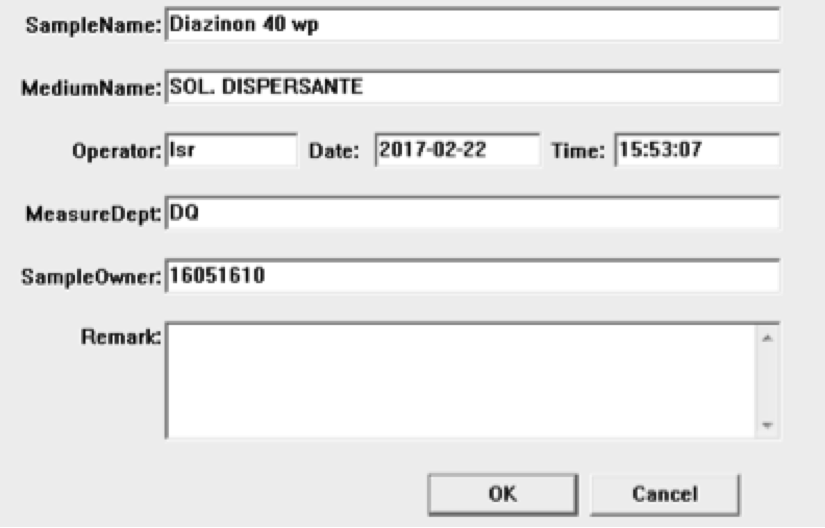
\includegraphics[width=0.5\linewidth]{img/aceptacion5.png}
	\caption{Datos ingresados}
	\label{fig:MarcoTeorico}
\end{figure}

\subsubsection{Procesar datos de estudio}

\begin{itemize}
	\item Se ajusta el instumento hasta que se encuentra en el nivel optimo, luego se ejecuta el análisis [Figura 2.27]
\end{itemize}

\begin{figure}[H]
	\centering
	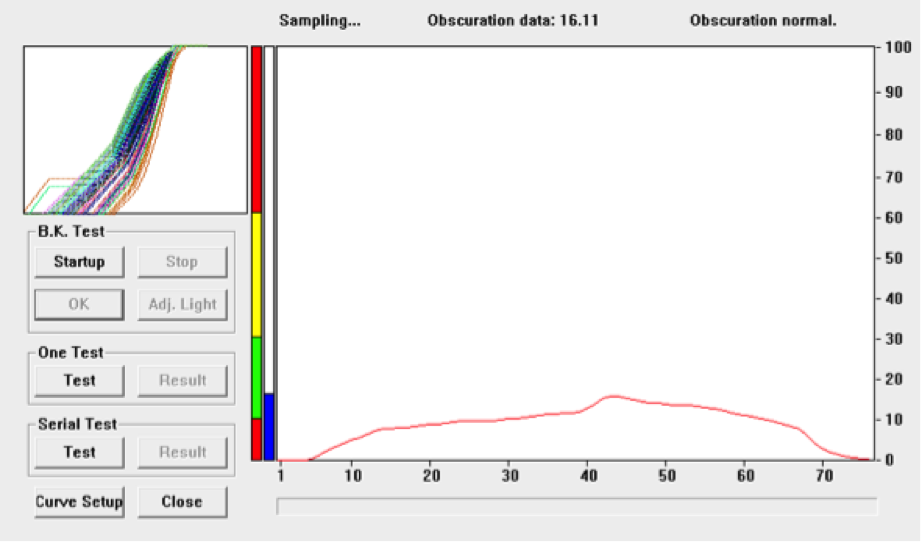
\includegraphics[width=0.4\linewidth]{img/aceptacion6.png}
	\caption{Proceso de datos}
	\label{fig:MarcoTeorico}
\end{figure}

\subsubsection{Resultados}

\begin{itemize}
	\item Se despliegan los resultados con el fin de comprar el valor obtenido con el especificado [Figura 2.26]
\end{itemize}

\begin{figure}[H]
	\centering
	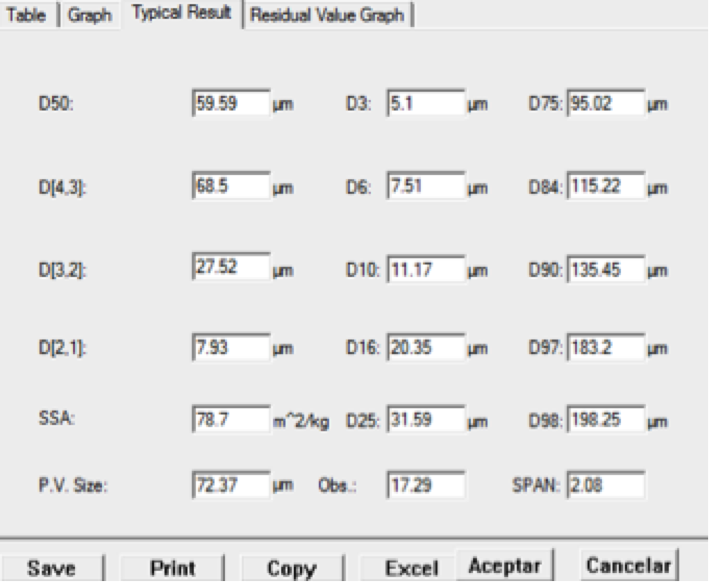
\includegraphics[width=0.4\linewidth]{img/aceptacion7.png}
	\caption{Vista de resultados}
	\label{fig:MarcoTeorico}
\end{figure}

\subsubsection{Estado de la validación: El sistema satisface el requerimiento}


\appendix
\chapter{Calificación de Diseño e Instalación}

En esta etapa de la validación se verifico que los sistemas contaran con los protocolos de integridad de datos y control de acceso. Ademas se aseguro que la infraestructura ocupada en la implementación de las soluciones inspeccianadas cumpliese con los requisitos operativos recomendados y definidos por el fabricante. Certificando que los aspectos clave del equipo y los necesarios para la instalación estén conforme a los estandares actuales.

\subsubsection{Aspectos inspeccionados}

\begin{itemize}
\item \textbf{Sistemas Operativos}: Los sistemas evaluados usan como plataforma de ejecución el sistema operativo recomendado (Windows 7 x64), los cuales se encuentran en optimas condiciones de funcionamiento.
\item \textbf{Memoria de acceso aleatorio}: La cantidad de memoria principal necesaria para ejecutar procesos y servicios cumple con lo recomendado por el fabricante.
\item \textbf{Memoria Secundaria}: La cantidad de memoria secundaria necesaria para ejecutar procesos y servicios cumple con lo recomendado por el fabricante.
\item \textbf{Capacidad de proceso}: La capacidad de procesamiento cumple con lo establecido por el fabricante.
\item \textbf{Licencias de software}: Todas las licencias asociadas con el uso de Software privativo se encuentran vigentes.
\item \textbf{Integridad de datos}: Protocolo anexo (Ver aparado Anexos).
\item \textbf{Politicas de acceso}: Documento anexo (Ver apartado Anexo).
\end{itemize}

\subsubsection{Estado: Validado}

\chapter{Calificación de operación}

En esta etapa de la validación se aseguro que las funciones y métodos involucrados en la elaboracion, directa o indirecta, de productos cumpliera con las expectativas de funcionamiento. Para ello se ejecutaron pruebas de Software, a un nivel Funcional y Aceptación. A continuación se presentan los resultados:

\subsubsection{Pruebas Funcionales}
\begin{itemize}
\item \textbf{Agilent Openlab EZChrom:} 8 casos de prueba ejecutados, 8 pruebas aceptadas. 
\item \textbf{TotalChrom navigator:} 8 casos de prueba ejecutados, 8 pruebas aceptadas. 
\item \textbf{Bettersize:} 3 casos de prueba ejecutados, 8 pruebas aceptadas.
\end{itemize}

\subsubsection{Pruebas de aceptación}

\begin{itemize}
	\item \textbf{Agilent Openlab EZChrom:} El sistema cumple con el requerimiento planteado. 
	\item \textbf{TotalChrom navigator:} El sistema cumple con el requerimiento planteado. 
	\item \textbf{Bettersize:} El sistema cumple con el requerimiento planteado.
\end{itemize}


\subsubsection{Estado: Validado}

